\chapter{Methodology}

The typical procedure for performing deep neural network molecular dynamics (MD) simulations is as follows:

\begin{itemize}
    \item \emph{Data Exploration}. Before training a model, it is necessary to first provide inputs such as atom types, the simulation box, and atom coordinates. Initial trajectories were generated using Molecular Dynamics as implemented in LAMMPS~\cite{LAMMPS}. The many-body potential employed is based on a previously trained deep neural network potential (NNP) generated by Sanchez-Burgos et al.~\cite{sanchez2023deep}.

          For the MD simulation, a system size of 192 water molecules was used for both the bulk and interface systems, as shown in Figure~\ref{fig:cryst_sctruct}. The temperature was varied from 300 K to 600 K. The simulation profile for the bulk system was as follows: an NPT ensemble at 1 bar for 2 ns, followed by a ramp from 1 bar to 10,000 bar over 10 ns. For the interface system, the simulation was conducted in the NVT ensemble for 10 ns, with the box size based on the average length of the corresponding bulk system at a given temperature and pressure of 1 bar. A vacuum was introduced to create a total length of 50 \r{A} in the direction normal to the interface. For both systems, a Nosé-Hoover thermostat with a relaxation time of 20 fs and a Nosé-Hoover barostat with a relaxation time of 200 fs were applied. The equations of motion were integrated using the time-reversible, measure-preserving Verlet and rRESPA integrators derived by Tuckerman et al.~\cite{Tuckerman2006}, with a simulation time step of 0.2 fs.

          \begin{figure}[tbhp]
              \centering
              \begin{subfigure}{0.42\textwidth}
                  \centering
                  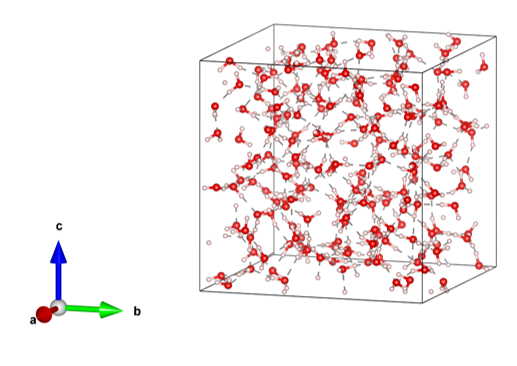
\includegraphics[width=0.75\textwidth]{bulk}
                  \caption{}
                  % \label{fig:}
              \end{subfigure}
              % \hfill
              \begin{subfigure}{0.42\textwidth}
                  \centering
                  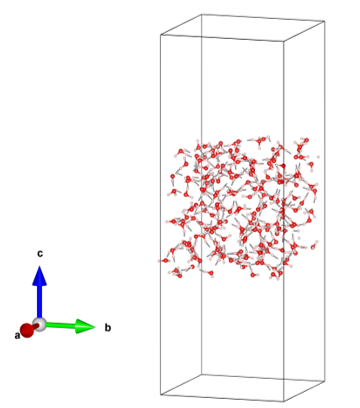
\includegraphics[width=0.75\textwidth]{interface}
                  \caption{}
                  % \label{fig:}
              \end{subfigure}
              \hfill
              \caption{Typical configurations for (a) bulk and (b) interface
                  systems.}\label{fig:cryst_sctruct}
          \end{figure}

    \item \emph{Data Labeling}.
          The trajectories were then labeled with their energy, force, and pressure tensor using Density Functional Theory (DFT) implemented in Quantum Espresso~\cite{QE-2009,QE-2017,QE-2020}. The Strongly Constrained and Appropriately Normed (SCAN) exchange-correlation functional is widely used in the study of water systems due to its excellent predictability in describing hydrogen bonds and van der Waals interactions~\cite{sun2015strongly, chen2017ab}. However, in this study, the SCAN functional tends to be numerically unstable when applied to systems with interfaces. Therefore, a similar but more accurate and numerically efficient r$^2$SCAN meta-generalized gradient approximation~\cite{Furness2020} was used instead. Optimized Norm-Conserving Vanderbilt pseudopotentials~\cite{hamann2013optimized} were employed, with an energy cutoff of 130 Ry and an SCF convergence threshold of \num{1e-6} Ry.

    \item \emph{Training}.
          The labeled frames were then fed into the DeePMD-kit code~\cite{wang2018deepmd,zeng2023deepmd,lu2021,zhang2018end} for the training of deep neural network potentials. A total of 1200 original bulk frames and 1000 original interface frames were used as training data. The training follows a typical two-neutral network architecture. First, atomic configurations are processed by an embedding network with three layers consisting of 25, 50, and 100 neurons each. The embedding uses the two-body smooth-edition scheme~\cite{zhang2018end} that conserves radial and angular information within a cutoff radius of 6 \r{A}. A switching function was applied for atoms beyond 5.5 \r{A} to ensure a smooth cutoff. Then, the atomic descriptors are built and used as input to a fitting network with three layers of 250 neurons each, which outputs a scalar quantity such as energy. The parameters of the neural network are set during the training procedure by minimizing a loss function based on the mean squared error of the total energy and atomic forces predicted by the network compared to the reference data. The minimization started with a large prefactor on the forces and ended with equal prefactors for both forces and energies. The iterative minimization was performed with a total of 3 million batches and a learning rate that exponentially decayed from \num{1e-3} to \num{3.5e-8}. Once the training is finished, the trained neural network will be ``frozen'' or saved into a protobuf (.pb) file that can be used as a many-body potential during MD simulations.



    \item \emph{Testing}. The neural network potential was tested by
          comparing results predicted by the NN potential with	  the results
          of DFT
          calculation on the validation datasets.

    \item \emph{Run MD}.
          Once the NN model was deemed satisfactory, one could perform molecular dynamics simulations using the trained neural network potential to predict the system's properties of interest. Equilibration was carried out for the first 2 ns, and the production run was performed for 10 ns.

    \item \emph{Check Deviation}.
          It is possible that during stochastic gradient descent runs, the NN model may reach different local minima. Hence, a common procedure is to train multiple similar models with different initializations by providing a random seed. These models will be used to run MD simulations, and deviations among these models will be compared. A larger deviation in structural properties (the default being atomic force) indicates less accuracy of the models. Using this criterion, a few trajectories with a maximum force standard deviation within the thresholds of 0.8 \unit{eV/\angstrom} and 1.5 \unit{eV/\angstrom}, respectively, will be selected for the next iteration. Each iteration will involve data labeling, and the new data will be combined with the initial data and data generated in previous iterations for further training. This process is called active learning. In this work, five iterations were applied to the bulk systems, resulting in a total of 6080 training frames.

    \item \emph{Obtain relevant properties}.
          Once the MD simulation is finished, one can compute properties of the system such as density, surface tension, and dipole orientation. The mass density was fitted according to the formula~\cite{sanchez2023deep}

          \begin{equation} \rho(z) = \frac{\rho_l + \rho_v}{2} - \frac{\rho_l - \rho_v}{2} \tanh\left(\frac{z - z_0}{d}\right) \label{eq:fit_dens}
          \end{equation}

          where $\rho_l$ and $\rho_v$ are the coexistence liquid and vapor densities, respectively, $z_0$ is the position of the interface, and $d$ is its thickness. For $\rho_l$ much greater than $\rho_v$, the thickness $d$ is roughly approximated as the distance between the location where the average density is 50\% of the bulk value and the location where it is 12\% of the bulk value.

          The surface tension can be calculated using the Kirkwood-Buff equation~\cite{kirkwood1949}, given by

          \begin{equation} \gamma = \frac{L_z}{2} \left[ \expval{P_{zz}} - \frac{1}{2} \left( \expval{P_{xx}} + \expval{P_{yy}} \right) \right] \label{eq:surf_tens}
          \end{equation}

          where $\expval{P_{\alpha \beta}}$ is the $\alpha \beta$th element of the pressure tensor, and $L_z$ is the total length of the box in the direction normal to the surface. The pressure tensor is computed by~\cite{thompson2009general}

          \begin{equation} P_{\alpha \beta} = \frac{1}{V} \sum_i^N m_i v_{i\alpha} v_{i\beta} + \frac{1}{V} \sum_i^{N'} R_{i\alpha} F_{i\beta} \end{equation}

          where $V$ is the volume, $N$ is the number of atoms, $N'$ includes atoms in the neighboring image cells, $m_i$ is the mass of the $i$th atom, and $v_{i\alpha}$, $R_{i\alpha}$, and $F_{i\alpha}$ are the velocity, position, and force of the $i$th atom in the $\alpha$ direction, respectively. The first term is related to the kinetic energy, while the second term is related to the virial.


\end{itemize}
